\section{Does the Qualified Design Pay? (RQ3)}
\label{sec:cost}
\subsection{RTX: deployment gain and speculative increment}
The RTX comparison separates two decisions before measuring their benefit (Figure~\ref{fig:cost}A). Ordinary target-only $R$ uses mask 0/UB1; matched target-only $M$ uses mask 3/UB4; speculative $C$, also denoted $C_3$, adds a draft at $k=3$ on that path. A fourth condition, $C_{15}$, constrains all phases. Each of four balanced rounds uses a separate resident process for each condition, with one excluded warmup and 24 formal requests per process. Condition and task orders rotate and recorded cache reuse is zero. The comparisons share tasks and a campaign, without sharing one simultaneous resident process.

In Table~\ref{tab:rtx_cost} and Figure~\ref{fig:cost}B,C, generation speed is $1.170\times$ ordinary and $1.169\times$ matched target-only, with 22/24 tasks faster in either comparison. Resident-request speed is $1.742\times$ ordinary but $1.035\times$ matched. The target-only path change itself gives $R/M=1.683\times$ request speed. Thus most of the measured deployment improvement is already available without a draft; $1.742\times$ describes the complete change, whereas $1.035\times$ is the speculative increment on the matched path.

% Generated by scripts/reconstruct.py from frozen exports.
\begin{table}[ht]\centering\small
\caption{RTX frozen expansion paid ratios: 24 task medians, four repeats. Gen. denotes generation; Request denotes resident request. Intervals describe task resampling. $C_3$ is mask 3 speculation.}\label{tab:rtx_cost}
\setlength{\tabcolsep}{4pt}
\begin{tabular}{@{}llrr@{}}\toprule
Ratio & Timer & Speed & 95\% interval\\\midrule
$R$/$C_3$ & Gen. & 1.170 & [1.117,1.218]\\
$R$/$C_3$ & Request & 1.742 & [1.655,1.827]\\
$M$/$C_3$ & Gen. & 1.169 & [1.117,1.217]\\
$M$/$C_3$ & Request & 1.035 & [1.005,1.063]\\
$R$/$M$ & Gen. & 1.001 & [0.995,1.008]\\
$R$/$M$ & Request & 1.683 & [1.590,1.766]\\
\bottomrule\end{tabular}

\end{table}


\begin{figure*}[t]
\centering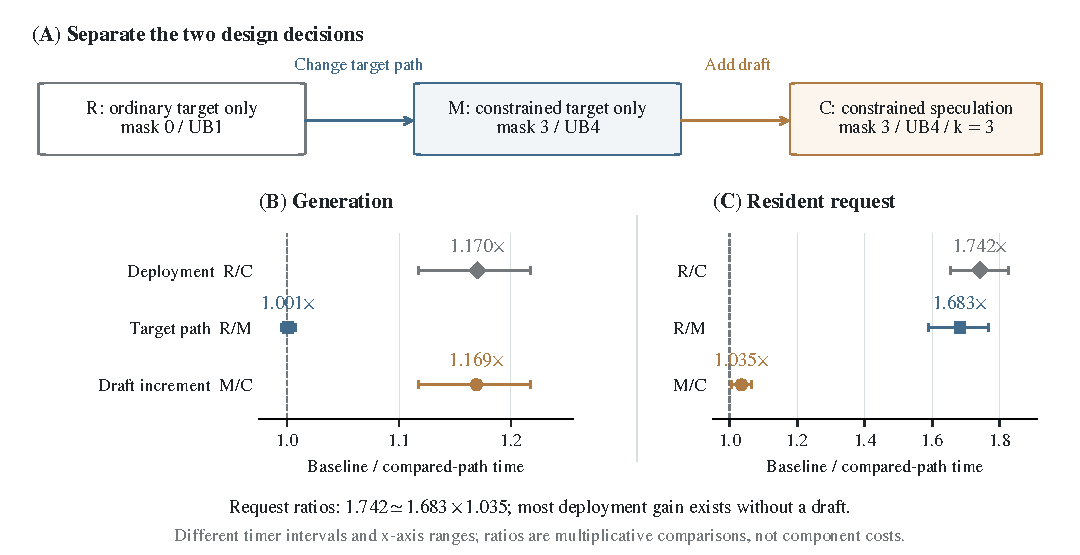
\includegraphics[width=\linewidth]{figures/figure_4_paid_cost.pdf}
\caption{Deployment gain and incremental draft benefit. (A) $R$ is ordinary target-only execution, $M$ the repaired target-only path, and $C$ speculation on that path. (B,C) Geometric means of 24 task ratios formed from four-repetition absolute-time medians; bars show descriptive 95\% task-bootstrap intervals. A ratio above one favors the denominator. Generation and resident-request timers use different intervals and axis ranges. Request ratios satisfy $R/C=(R/M)(M/C)$; this multiplication separates comparisons rather than component costs.}
\label{fig:cost}
\end{figure*}

The identity in Equation~\ref{eq:identity} holds for all 48 task-timer cells and both aggregate timers. Generation $R/M$ is near parity while request $R/M$ is much larger. The target-path change affects prefill microbatch/attention behavior and continuation capacity jointly, and the timer boundaries differ. Their contrast cannot allocate a measured host, attention, KV or synchronization share. A faster qualified ordinary implementation could also narrow the deployment benefit: the registered $R$ is an executed reference, not a proven fastest ordinary decoder.

\subsection{Task variation and session uncertainty}
Figure~\ref{fig:tasks}A,B shows all 24 tasks in the same request-sorted order and scale. Generation improves on 22/24 tasks, but request time improves on only 17/24. Seven tasks regress against matched execution, despite all 24 being faster than ordinary request cost. The average request gain therefore does not justify an unconditional per-task acceleration claim.

The within-round matched-request geometric means in Figure~\ref{fig:tasks}C are 1.029, 0.940, 1.052 and 1.044: round 2 reverses direction. These round summaries differ from the geometric mean formed after taking each task's four-repetition absolute-time medians. The descriptive task-bootstrap interval for that median-based aggregate lies above one, but does not remove the observed round reversal or estimate independent session/day uncertainty.

\begin{figure*}[t]
\centering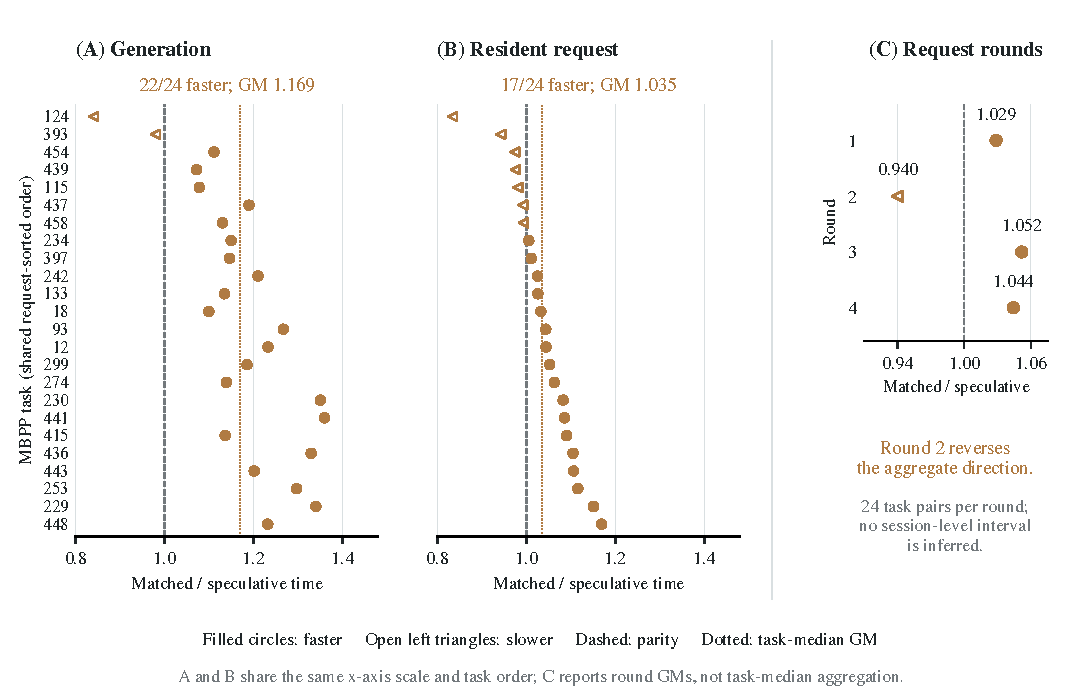
\includegraphics[width=\linewidth]{figures/figure_5_task_variation.pdf}
\caption{Variation behind the matched RTX benefit. (A,B) All 24 tasks share order and scale; ratios use four-repetition absolute-time medians. Generation improves on 22/24 and request time on 17/24. Filled circles denote faster speculation and open left triangles slower speculation, separately for each timer. Dashed lines mark parity; dotted lines mark task-median geometric means. (C) Geometric means within four request rounds, with reversal in round 2. Round summaries are not the task-median estimator or a session-level uncertainty interval.}
\label{fig:tasks}
\end{figure*}

The operating point is qualified and positive in aggregate, with a small, uneven request increment. Separate resident sessions, laptop scheduling and thermal variation can affect that estimate; balanced order and task medians do not eliminate session confounding. The larger generation gain applies to its defined interval rather than replacing the request result. Independent session/day replication would be needed to assess stable deployment acceleration.

A separate serial resident-reset study checks whether the anchor preserves output when reused across requests. Two orders retain the registered reference after target-state reset, with matched generation/request speeds about $1.181\times/1.039\times$. This supports finite reset semantics for the original $k=3$/UB4 recipe, without establishing concurrency, throughput or resident qualification of the widened draft. These rows are not pooled with the expansion.

\subsection{Fixed UB: wider drafting qualifies but becomes slower}
The fixed-UB experiment tests the cost of widening a qualified draft. Unlike the joint $k$/UB geometry sweep, this experiment fixes UB4 and mask 3 while testing $k=3,5,7$ on 24 now-exposed MBPP inputs and four exposed HumanEval probes. Each width qualifies in two repetitions. The highest passing width, $k=7$, is then measured in a separate capture-off arm: four conditions, four repetitions and 448 formal requests. Qualification timings do not select the width by speed.

Relative to $k=3$, $k=7$ gives $0.829\times$ generation and $0.890\times$ request speed. Against matched target-only it gives $0.997\times/0.950\times$, whereas the anchor gives $1.203\times/1.068\times$ in this campaign. Ordinary same-width speculation fails its output gate, so its timing cannot serve as qualified speed evidence. For these inputs and this configuration, the measured anchor is preferable to the wider qualified draft.

Caller reduction does not reduce all recorded work. Drafted tokens rise from 3,528 to 5,392, while accepted draft tokens rise from 2,772 to 3,192. Separate captured qualification sessions record target continuation caller counts falling from 305 to 199 but micrographs increasing from 305 to 397. These counts include their own warmups and forced synchronization; they cannot be divided into formal timing to create a component profile. Micrographs are not CUDA kernel launches, and no unique slowdown component is isolated.

At $k=7$, matched generation/request speed is $0.953\times/0.919\times$ on 24 MBPP inputs and $1.308\times/1.164\times$ on four HumanEval probes. Four exposed probes do not validate an online routing rule. Supplement \S S4.3 retains these partitions and the longer-cap checks under their own timers and panels.

\subsection{B570: repair improves an old path but loses to strong baselines}
The B570 repair's formal four-condition matrix contains 119/120 payloads; old N1's first-round MBPP/400 record is missing after an infrastructure interruption. Its time remains unknown, without imputation or a scientific rerun. Ordinary $R$, matched $M$ and candidate $C$ each have 30 complete responses and 15 two-round task-median pairs. Old-N1 comparisons use 14 complete pairs.

The candidate fails the latency objective against both strong baselines (Table~\ref{tab:b570_cost}). Generation/whole-request speed is $0.283\times/0.201\times$ against ordinary $R$ and $0.286\times/0.206\times$ against matched target-only. Both baselines are faster in every available paired round. The target-only paths are close in cost, with $R/M=0.989\times/0.979\times$; the roughly fivefold candidate request cost is therefore not explained by the target-path consistency constraint alone.

% Generated by scripts/reconstruct.py from frozen exports.
\begin{table}[ht]\centering\small
\caption{B570 paid baseline/candidate task-median ratios. $n$ counts complete two-round task pairs: 15 for $R/C$, $M/C$ and $R/M$, and 14 for old N1/$C$. Gen., Request and Host denote generation, whole request and host-observed time. The missing old-N1 task is not imputed; raw suffix work stays charged.}\label{tab:b570_cost}
\setlength{\tabcolsep}{3pt}
\begin{tabular}{@{}lrrrr@{}}\toprule
Ratio & $n$ & Gen. & Request & Host\\\midrule
$R/C$ & 15 & 0.283 & 0.201 & 0.202\\
$M/C$ & 15 & 0.286 & 0.206 & 0.206\\
Old N1/$C$ & 14 & 3.993 & 2.634 & 2.633\\
$R/M$ & 15 & 0.989 & 0.979 & 0.979\\
\bottomrule\end{tabular}

\end{table}


Against the prior old-N1 frontend, the candidate improves generation/request speed by $3.993\times/2.634\times$ over 14 pairs. That improvement is relative to a slow frontend and does not establish a benefit over ordinary deployment. MBPP/245 also reverses the old-path whole/host request comparison in round 2. Endpoint recovery and aggregate improvement do not guarantee improvement in every round.

The endpoint contract retains all online work. Candidate endpoint IDs total 1,150 while raw IDs total 1,176, with all 26 suffix IDs charged. The records contain 888 drafted and 702 accepted tokens, and target/draft continuation caller-token totals of 1,332/1,362. These quantities describe different parts of the transaction; endpoint equality does not assert raw suffix equality. Removing witness readbacks, an extra context and handoff improves the frontend, but phase reservation, synchronization, drafting and rollback remain. Without a full component profile, the remaining bottleneck cannot be assigned uniquely. The paid decision is to reject this candidate for latency against $R$ and $M$.

\subsection{Global serialization, control, and draft-side limits}
Global serialization can recover output while increasing cost. An earlier RTX arm qualifies 57/57 arrays on 19 exposed tasks but achieves $0.677\times$ target-only speed, with descriptive interval $[0.662,0.692]$ and no task faster. Its synchronized post-prefill-to-slot-release timer includes instrumentation and logging. It is a separate negative operating point, not an earlier point on the expansion's server-generation curve; Supplement \S S6.4 retains the host amendment and preceding V3 stop.

The prospective M4 control campaign has 60 tasks, three conditions, three repeats and 540 requests under a post-prefill contract. Always speculation and Guard each qualify 180/180 direct-ID comparisons. Target-only/Always speed is $1.347\times$, but the paired secondary Guard/Always latency ratio is 1.027, with descriptive interval $[1.013,1.044]$: the measured guard is slower. A hindsight oracle choosing only target-only or Always offers about 0.069\% further geometric-mean latency reduction. This narrow two-action opportunity does not bound intra-request policies; the primary and secondary statistical streams remain distinct (Supplement \S S6.6).

On 358H, CPU/NPU drafting each qualifies 90 direct-ID comparisons but gives $0.734\times/0.352\times$ speed. With measured target work and committed progress fixed, eliminating every other nonnegative cost yields prompt-estimator ceilings of $0.837\times/0.845\times$. Even that idealization needs a uniform target-work reduction of at least 16.28\%/15.52\% to reach parity. Draft-only optimization cannot close this conditional budget; changing the target path or state interface requires new qualification and measurement. These are necessary budgets, not achieved optimizations or an impossibility result for NPUs (Supplement \S S6.7). M4 and 358H inform separate design decisions and do not replicate the RTX repair.
\FloatBarrier
